
\documentclass[letterpaper,11pt]{article}
\newlength{\outerbordwidth}
\pagestyle{empty}
\raggedbottom
\raggedright
\usepackage[svgnames]{xcolor}
\usepackage{framed}
\usepackage{times}
\usepackage{tocloft}
\usepackage{graphicx}
\usepackage{multirow}
\usepackage[utf8]{inputenc}
\usepackage{tabularx} 
\usepackage{hyperref}
\usepackage{pdfpages}
\title{VINIT_NARAYAN_JHA}
 
\setlength{\outerbordwidth}{3pt}  
\definecolor{shadecolor}{gray}{0.75}   
\definecolor{shadecolorB}{gray}{0.93}  
 
\setlength{\evensidemargin}{-0.25in}
\setlength{\headheight}{0in}
\setlength{\headsep}{0in}
\setlength{\oddsidemargin}{-0.25in}
\setlength{\paperheight}{11in}
\setlength{\paperwidth}{8.5in}
\setlength{\tabcolsep}{0in}
\setlength{\textheight}{9.5in}
\setlength{\textwidth}{7in}
\setlength{\topmargin}{-0.3in}
\setlength{\topskip}{0in}
\setlength{\voffset}{0.1in}

\newcommand{\resitem}[1]{\item #1 \vspace{-2pt}}
\newcommand{\resheading}[1]{\vspace{8pt}
  \parbox{\textwidth}{\setlength{\FrameSep}{\outerbordwidth}
    \begin{shaded}
\setlength{\fboxsep}{0pt}\framebox[\textwidth][l]{\setlength{\fboxsep}{4pt}\fcolorbox{shadecolorB}{shadecolorB}{\textbf{\sffamily{\mbox{~}\makebox[6.762in][l]{\large #1} \vphantom{p\^{E}}}}}}
    \end{shaded}
  }\vspace{-5pt}
}
\newcommand{\ressubheading}[4]{
\begin{tabular*}{6.5in}{l@{\cftdotfill{\cftsecdotsep}\extracolsep{\fill}}r}
  \textbf{#1} & #2 \\
  \textit{#3} & \textit{#4} \\
\end{tabular*}\vspace{-6pt}}
 
\begin{document}

\begin{tabular*}{7in}{l@{\extracolsep{\fill}}r}
  & \multirow{4}{*}{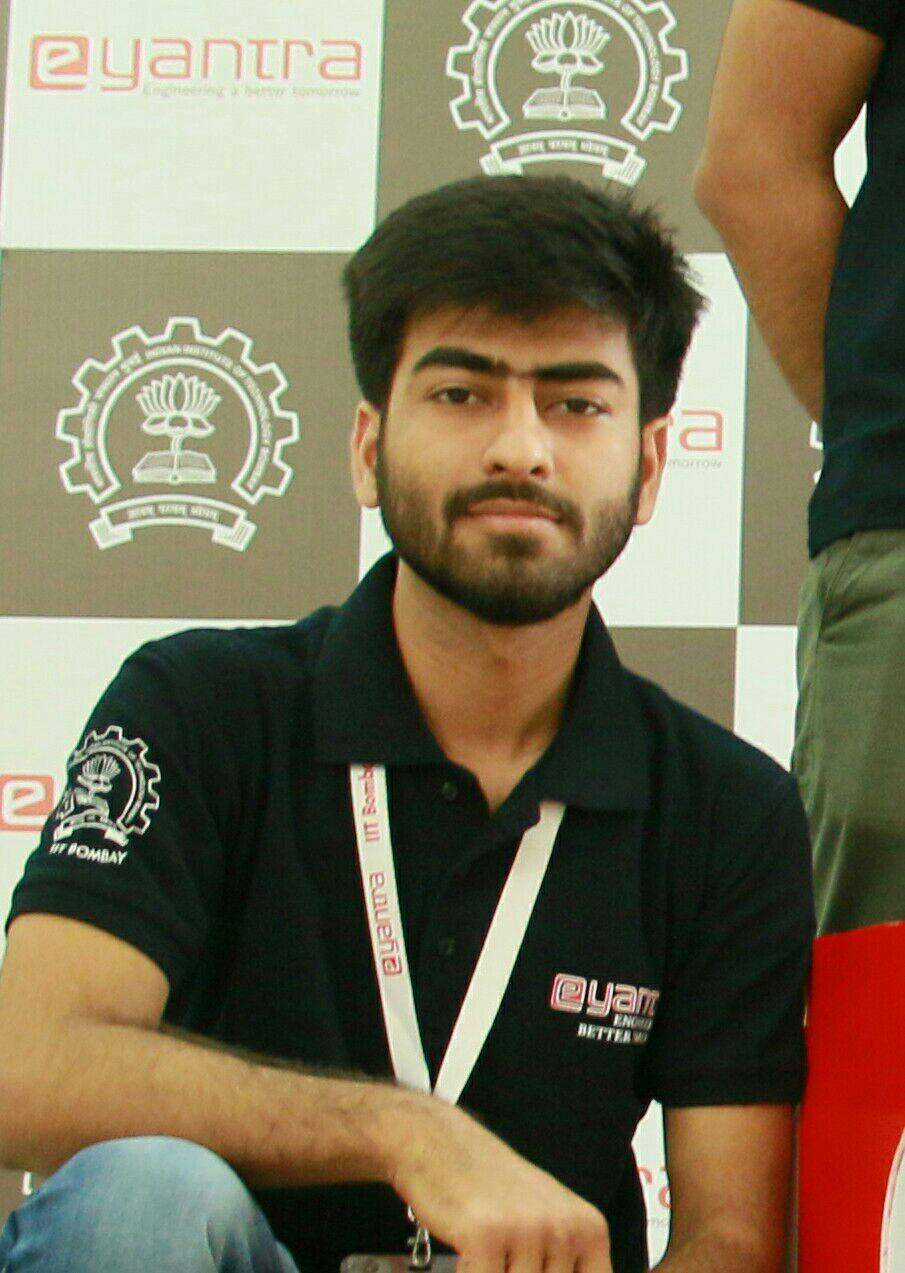
\includegraphics[scale=0.1]{azhar.jpg}}\\
  & \\
%-----------------------------------------------------------  
  \textbf{\Large Mohammad Azharuddin } & \\\\
  Email: azharcaptain20@gmail.com & \\
  Contact: 7889081853  \\
  Address: Q.No 3137 sector 47 chandigarh,160047  \\

\end{tabular*}
\\


%%%%%%%%%%%%%%%%%%%%%%%%%%%%%%
\resheading{Career Objective}
%%%%%%%%%%%%%%%%%%%%%%%%%%%%%%
  \begin{center}
  \parbox{6.762in}{3rd year B.E student of Electronics and Communication at University Institute of Engineering and Technology, Panjab University. Inquisitive, hard-working and consistent. Very interested in making projects related to electronics and Robotics and looking forward for an internship in Robotics.}
  \end{center}
  
%%%%%%%%%%%%%%%%%%%%%%%%%%%%%%
\resheading{Education}
%%%%%%%%%%%%%%%%%%%%%%%%%%%%%
\begin{center}
\renewcommand{\arraystretch}{2.0}
\begin{tabular}{ | c | c| c | c | c | }
\hline
Degree  & College/School & University & Passing Year &  Pass Percentage \\ 
\hline
10th Class & Kendriya Vidyalaya sector 31 chandigarh & CBSE(Board) & 2014 & 10 CGPA \\ 
\hline
12th Class & Kendriya Vidyalaya Sector-31 Chandigarh & CBSE(Board) & 2016 & 89 \\ 
\hline
BE ECE(3rd year) & University Institute of Enginnering and Technology & Panjab University & 2020 & 7.85(CGPA) \\
\hline
\end{tabular}
\end{center}

%%%%%%%%%%%%%%%%%%%%%%%%%%%%%%
\resheading{Projects}
%%%%%%%%%%%%%%%%%%%%%%%%%%%%%%
 \begin{enumerate}

\item \textbf {Autonomous Crow Robot:}
Made the robot from scratch which works like thirsty crow in the jungle, picking the pebbles(metallic balls) and placing in the the pitcher(specific area on the area).This story is brought into reallity on the screen using augmented Reality Technology. 
\begin{itemize}
\item \textbf{Technology/Tools:} Embedded C, OpenGL, Path planning, OpenCV, XBee communication, Python 
\end{itemize}
\begin{itemize}
\item \textbf{Youtube Link:} https://www.youtube.com/watch?v=DdPGsyRq_lw&feature=youtu.be
\end{itemize}

\item \textbf {Wire Extrusion:}
Involved with the electronics aspect of Extrusion machine. Combined the working of three stepper motor used in the machine on one single microcontroller(Arduino nano) and made a seperate module for this. Contorlled The speed of the motors using the inbuilt timers of Arduino nano. Desined a mechanism for sweeping the wire on the spool(circular thing on which wire is wrapped) uniformly using a switch and interrupt. 

\begin{itemize}
\item \textbf{Technology/Tools:} Embedded C, Arduino IDE
\end{itemize}
\begin{itemize}
\item \textbf{Video link:} https://drive.google.com/open?id=1QfjfdG8ZZFpbYy9xYUHKUDQQ1lk6nkva
\end{itemize}

 
  \item \textbf{Bite Force(Collaboration with GMCH-32 Hospital):} 
Worked on developing a module for the doctors which can measure the force of teeth while the patient bites using the pressure sensor and determining  health, hygine, disease and recovery of the tooth after any surgery. Also I interfaced an OLED on the module, which shows values of pressure from the tooth at the time of bite and also the doctor can later recollect the values of the patients of which the bites have been taken later on also. This is done using the EEPROM memory of the Arduino nano.
% \end{itemize}
\begin{itemize}
\item \textbf{Technology/Tools:} Arduino IDE
\end{itemize}

\begin{itemize}
\item \textbf{Report link:} https://drive.google.com/open?id=18qXjPWVtBbSYwQGmHe48f0wIXmOOmh3-efq-MZuRBbI
\end{itemize}

 \item \textbf {Password Based Door Lock:}

Worked on Password Based Door Lock System using 8051 Microcontroller using Embedded C in Keil. 
% \end{itemize}
\begin{itemize}
\item \textbf{Technology/Tools:} Keil, Embedded C, 8051 development kit
\end{itemize}

\begin{itemize}
\item \textbf{Link:} https://drive.google.com/open?id=1YzH3cSRm4CVV6TAUyOUlbocSX6CXINPj
\end{itemize}



\item \textbf{Bus on Time(Currently working):}
 Made a device module which fitted on the bus, will keep sending the GPS location to the Google sheet using the nodeMCU. The coordinates send by the bus will now be fetched from the google sheet and then processes by the backend programme which will keep updating the bus location in the database of the programme and when any user wishes to know the position of the bus he will enter the bus no. and the bus current location will be shown to him. 
% \end{itemize}
\begin{itemize}
\item \textbf{Technology/Tools:} Arduino IDE, Javascript, Python, Sheetsu
\end{itemize}

 \end{enumerate}

%%%%%%%%%%%%%%%%%%%%%%%%%%%%%%
\resheading{Training and Internship}
%%%%%%%%%%%%%%%%%%%%%%%%%%%%%%
\begin{itemize}
    \item \textbf{Intern at DESIGN AND INNOVATION CENTER : Initiative By MHRD(Gov.of India) on collaborative research and innovation PU,Chandigarh, India \hfill{(Jun 18 - Aug 18)}\\}Learnt about the various inbuilt registers of the ATmega 328 and made a project using the timers and interrupts of Arduino.
\end{itemize}




\\
\begin{itemize}
\item \textbf{C Programming Training\hfill{(Jun 17 - Aug 17)}\\}Learnt fundamentals of programming 
\end{itemize}
\\

\begin{itemize}
\item \textbf{Training activity Under college Programme\hfill{(June 2017)}\\}Learnt Arduino, Motor Driver, Sensor Interfacing, Arduino IDE and made a project Automatic Floor cleaner which as the name suggest cleans the floor by interfacing with Ultrasonic sensor and DC motor
\end{itemize}

%%%%%%%%%%%%%%%%%%%%%%%%%%%%%%
\resheading{Research and Publications}
%%%%%%%%%%%%%%%%%%%%%%%%%%%%%%
  \begin{itemize}  \resitem{  None } 
 \end{itemize}
 

 
%%%%%%%%%%%%%%%%%%%%%%%%%%%%%%
\resheading{Websites work}
%%%%%%%%%%%%%%%%%%%%%%%%%%%%%%
\begin{itemize}
\item\textbf{Hackerrank : } https://www.hackerrank.com/azharcaptain20
\end{itemize}
\\
\begin{itemize}
\item\textbf{Hackerearth :} https://www.hackerearth.com/@mohammad557
\end{itemize} 
\\
\begin{itemize}
\item\textbf{Linkedin : } https://www.linkedin.com/in/mohammad-azharuddin-30a494147/
\end{itemize}


\resheading{Technical Skills}
%%%%%%%%%%%%%%%%%%%%%%%%%%%%%%
\begin{itemize}
\item\textbf{Software : } Embedded C, Python, C++, C, Atmel Studio
\end{itemize}
\\
\begin{itemize}
\item\textbf{Hardware :} Arduino, AVR mC, Spark V kit, Firebird V kit, Various Driver Modules and Sensor Modules \end{itemize} 
\\
\begin{itemize}
\item\textbf{General : } Data Structures, Algorithm
\end{itemize}

%%%%%%%%%%%%%%%%%%%%%%%%%%%%%%
\resheading{Soft Skills}
%%%%%%%%%%%%%%%%%%%%%%%%%%%%%%
\begin{enumerate}
    \item Problem solving
    \item Team work
    \item Team Leader
    \item  Always Learning attitue
\end{enumerate}


%%%%%%%%%%%%%%%%%%%%%%%%%%%%%%
\resheading{Extracurricular activities}
%%%%%%%%%%%%%%%%%%%%%%%%%%%%%%
\begin{itemize}
 \item Worked as a volunteer for Rotaract Club of UIET for an event 'Helping Run' which was organised for NGO Gur Asra Trust,Palsora. 
 \item Worked as volunteer in Marketing team of Goonj fest organized in UIET,PU 2017. 
\end{itemize}


%%%%%%%%%%%%%%%%%%%%%%%%%%%%%%
\resheading{Co-curricular activities}
%%%%%%%%%%%%%%%%%%%%%%%%%%%%%%
\begin{enumerate}
    \item Group leader of college electronics group : Embedded Group of UIET,PU
    \item Help to flourish electronics environment in college and e-Yantra Lab(initiative by IIT Bombay) in college
    \item Organized electronics hackathon on North India level.
\end{enumerate}

%%%%%%%%%%%%%%%%%%%%%%%%%%%%%%
\resheading{Personal Details}
%%%%%%%%%%%%%%%%%%%%%%%%%%%%%%
\begin{center}
\parbox{6.762in}{
 Father's Name: Riyaz Ali\\
Mother's Name: Tasneem\\
Sex: Male\\
Date of Birth: 20 February 1999\\
Nationality:   Indian\\
Martial Status: Not Married\\
}
\end{center}

%%%%%%%%%%%%%%%%%%%%%%%%%%%%%%
\resheading{Reference}
%%%%%%%%%%%%%%%%%%%%%%%%%%%%%%
  \begin{itemize}
  \resitem{  None } 
 \end{itemize}

%%%%%%%%

%%%%%%%%%%%%%%%%%%%%%%
\resheading{Declaration}
%%%%%%%%%%%%%%%%%%%%%%%%%%%%%%
I do hereby declare that above particulars of information and facts stated are true, correct and complete to the best of my knowledge and belief.\\

%%%%%%%%%%%%%%%%%%%%%%%%%%%%%%
\resheading{Date}
%%%%%%%%%%%%%%%%%%%%%%%%%%%%%%
17\textsuperscript{th}-April-2019

\end{document}